
% Appendix C
\chapter{Appendix C}
%\chapter{Additional curves for selected industry } % Main appendix title


%\label{AppendixC} % 



% 1
\section{Figure 5.3 with full Axis range}

\begin{figure}
    \centering
    \makebox[\textwidth][c]{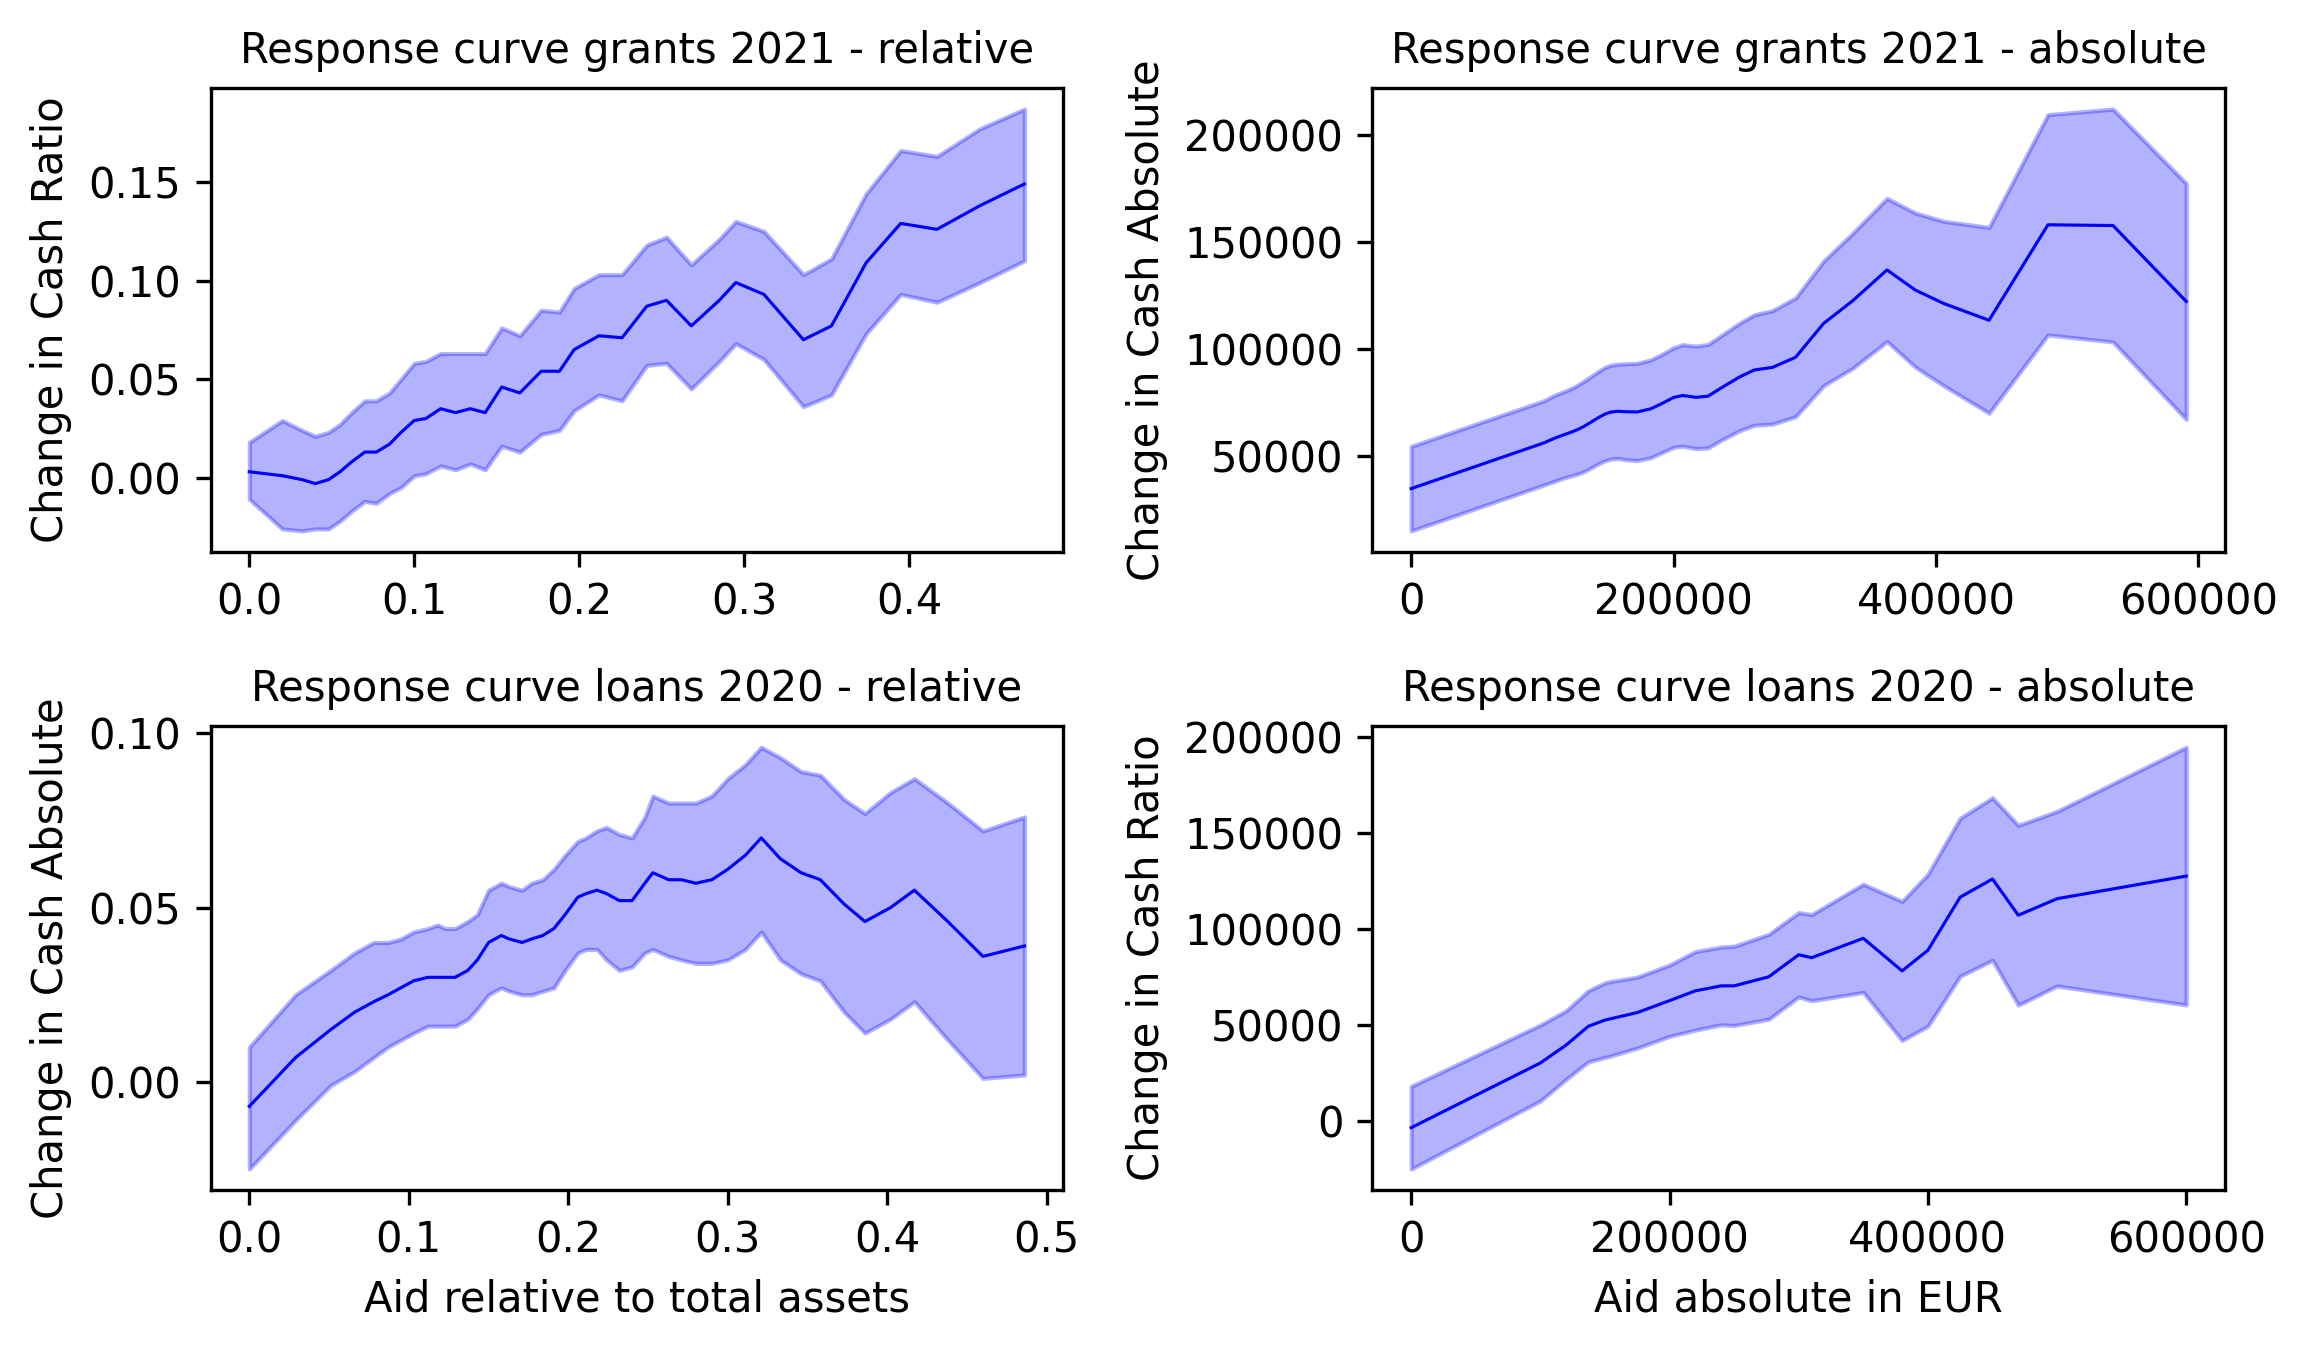
\includegraphics[width=1\columnwidth]{Figures/causal_curves1_raw.png}}
    
    \decoRule
    \caption[Response curves for grants and loans uncut]{Estimated Dose Response Functions, for liquidity (cash) from grants 2021 (top) and loans 2020 (bottom) in relative (left) and absolte (right) terms with 95\% Confidence Bands. For Binomial Distributed Data. The estimate of absolute variants used a lognormal GLM for the GPS estimation due to the different distribution of the variables.}
    \label{fig:Curve1raw}
\end{figure}


% 2
\section{Figure 5.4 with full Axis range}

\begin{figure}
    \centering
    \makebox[\textwidth][c]{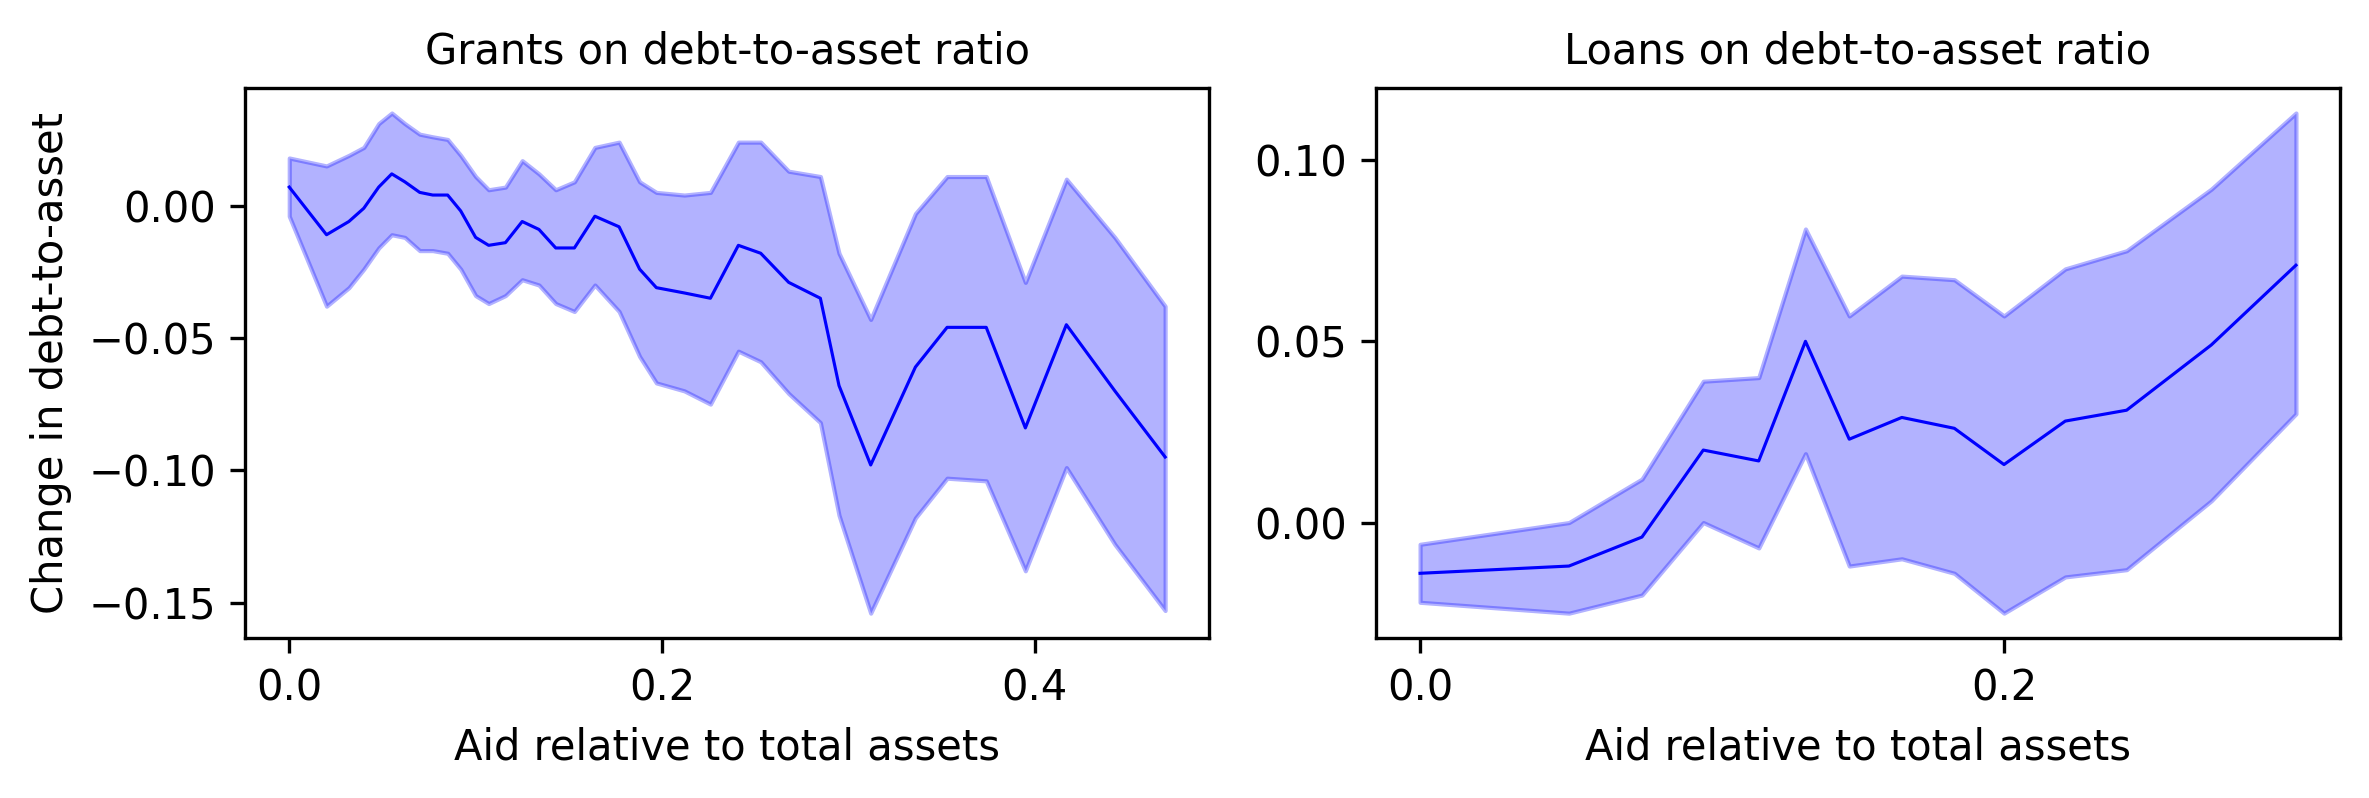
\includegraphics[width=1\columnwidth]{Figures/causal_curves2_raw.png}}
    
    \decoRule
    \caption[Response curves for indebtedness through aid uncut]{Estimated Dose Response Functions, for the debt-to-asset ratio from grants 2021 and loans 2021 in relative terms with 95\% Confidence Bands}
    \label{fig:Curve2raw}
\end{figure}



% 3
\section{Figure 5.5 with full Axis range}

\begin{figure}
    \centering
    \makebox[\textwidth][c]{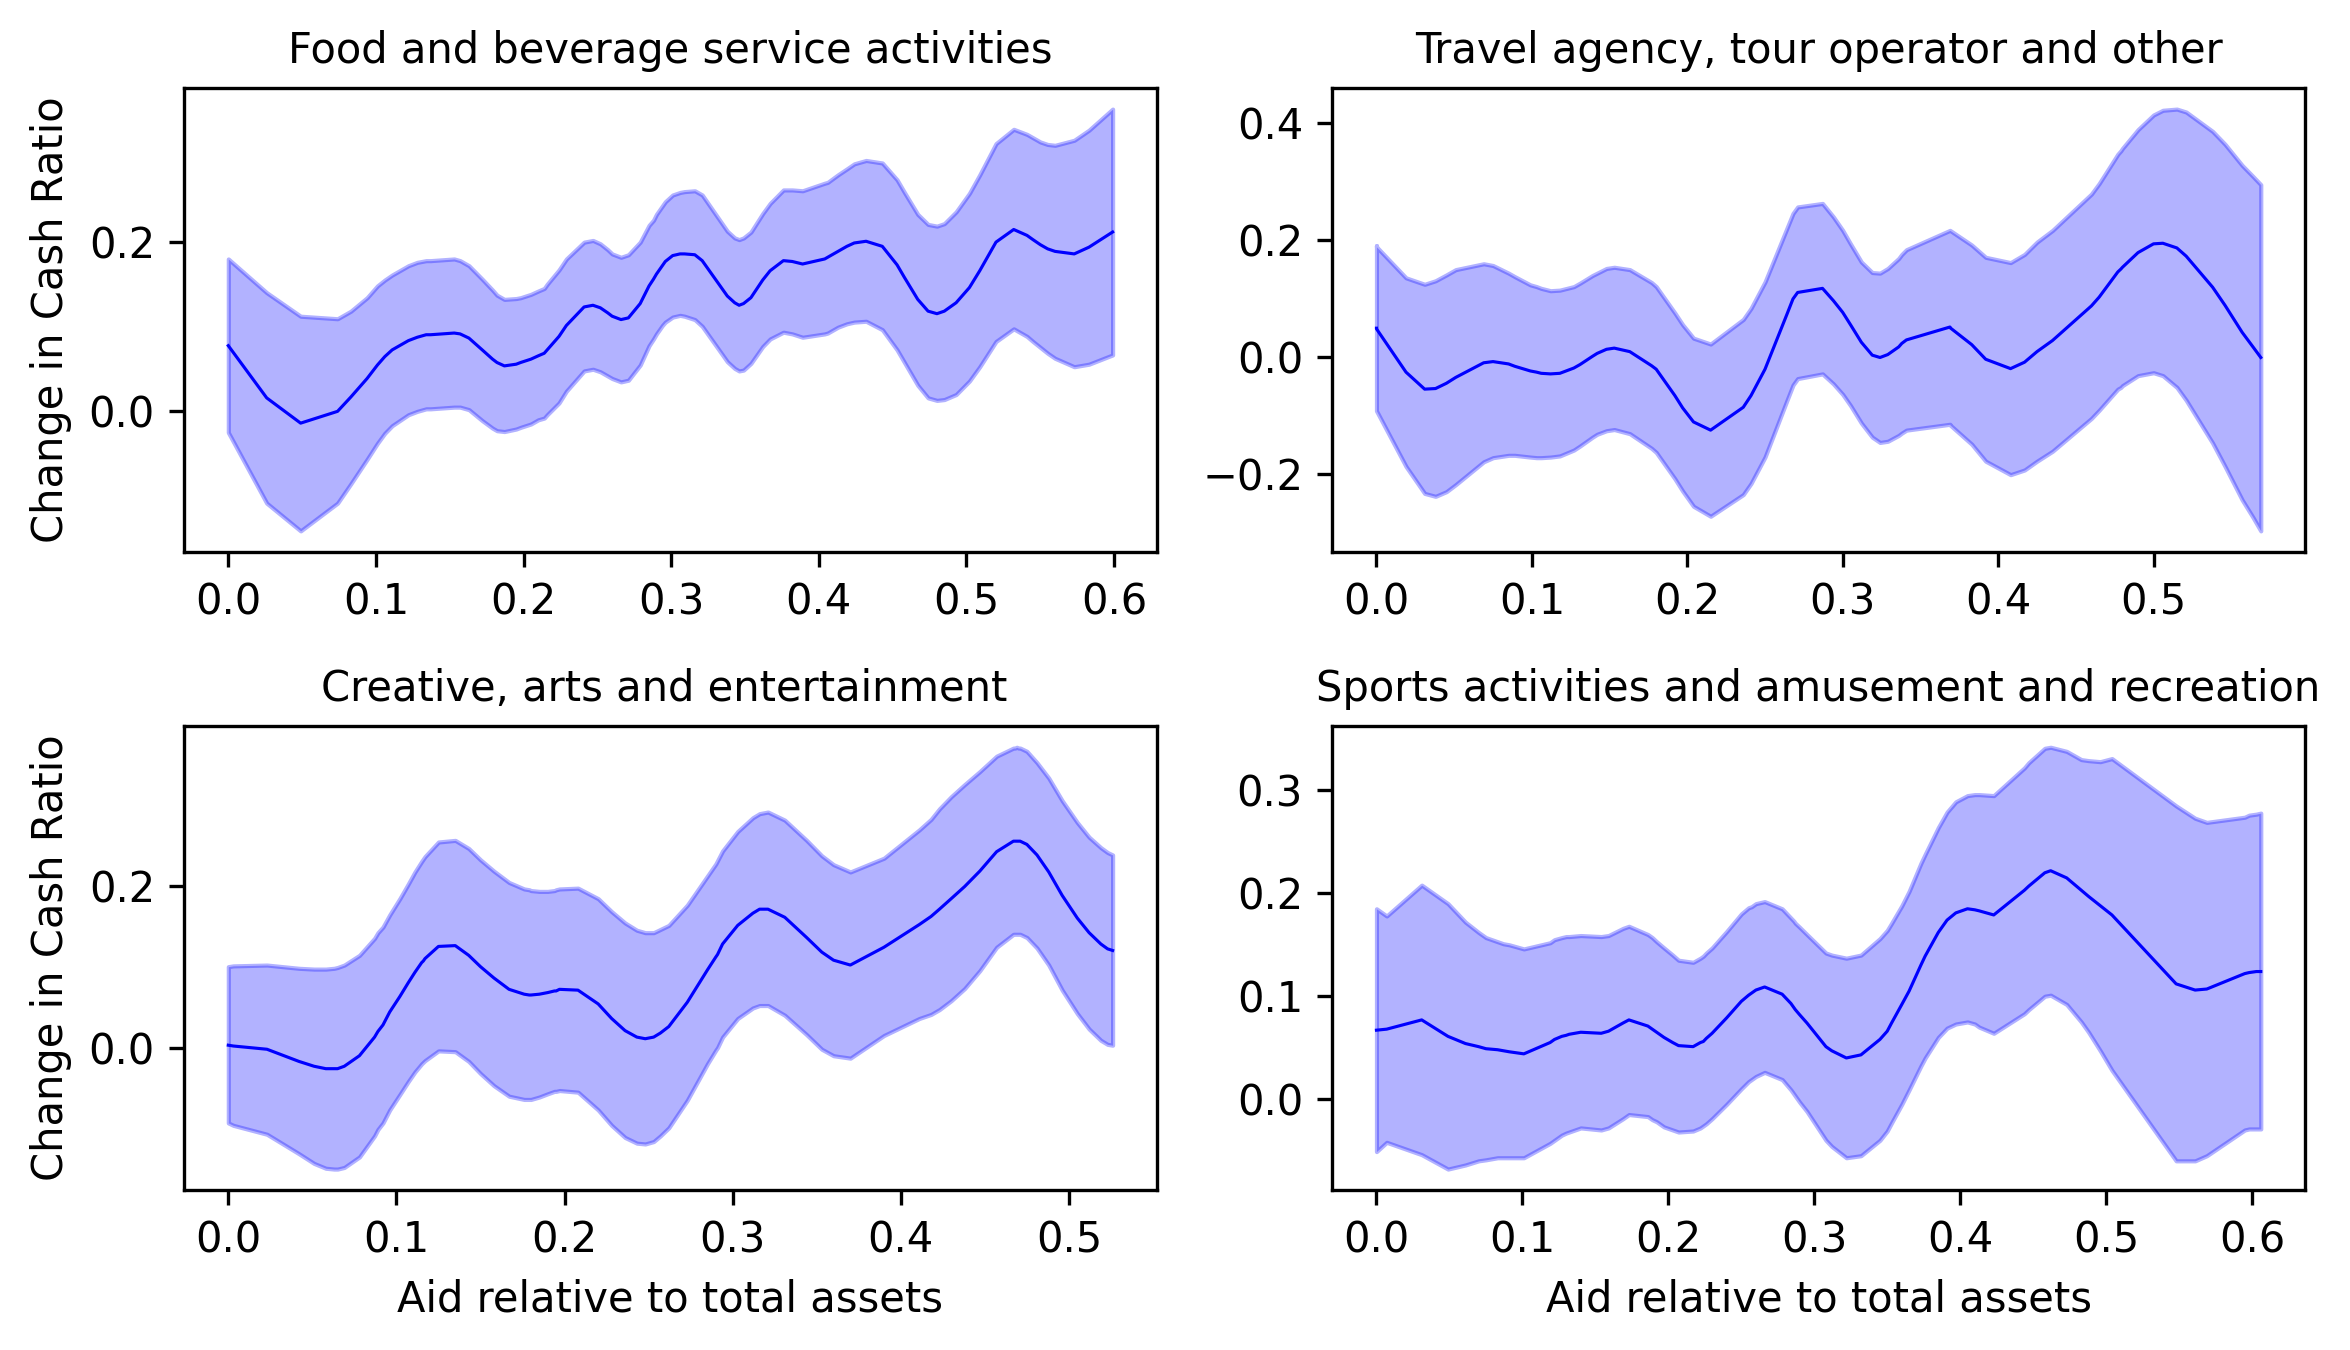
\includegraphics[width=1\columnwidth]{Figures/causal_curves_industries1_RAW.png}}
    
    \decoRule
    \caption[Response curves for liquidity through aid - by sectors 1 uncut]{Estimated Dose Response Functions, for the cash ratio from grants 2021 in selected industries in relative terms with 95\% Confidence Bands}
    \label{fig:Curve3raw}
\end{figure}



% 4
\section{Dose curves from addtional industries}

\begin{figure}
    \centering
    \makebox[\textwidth][c]{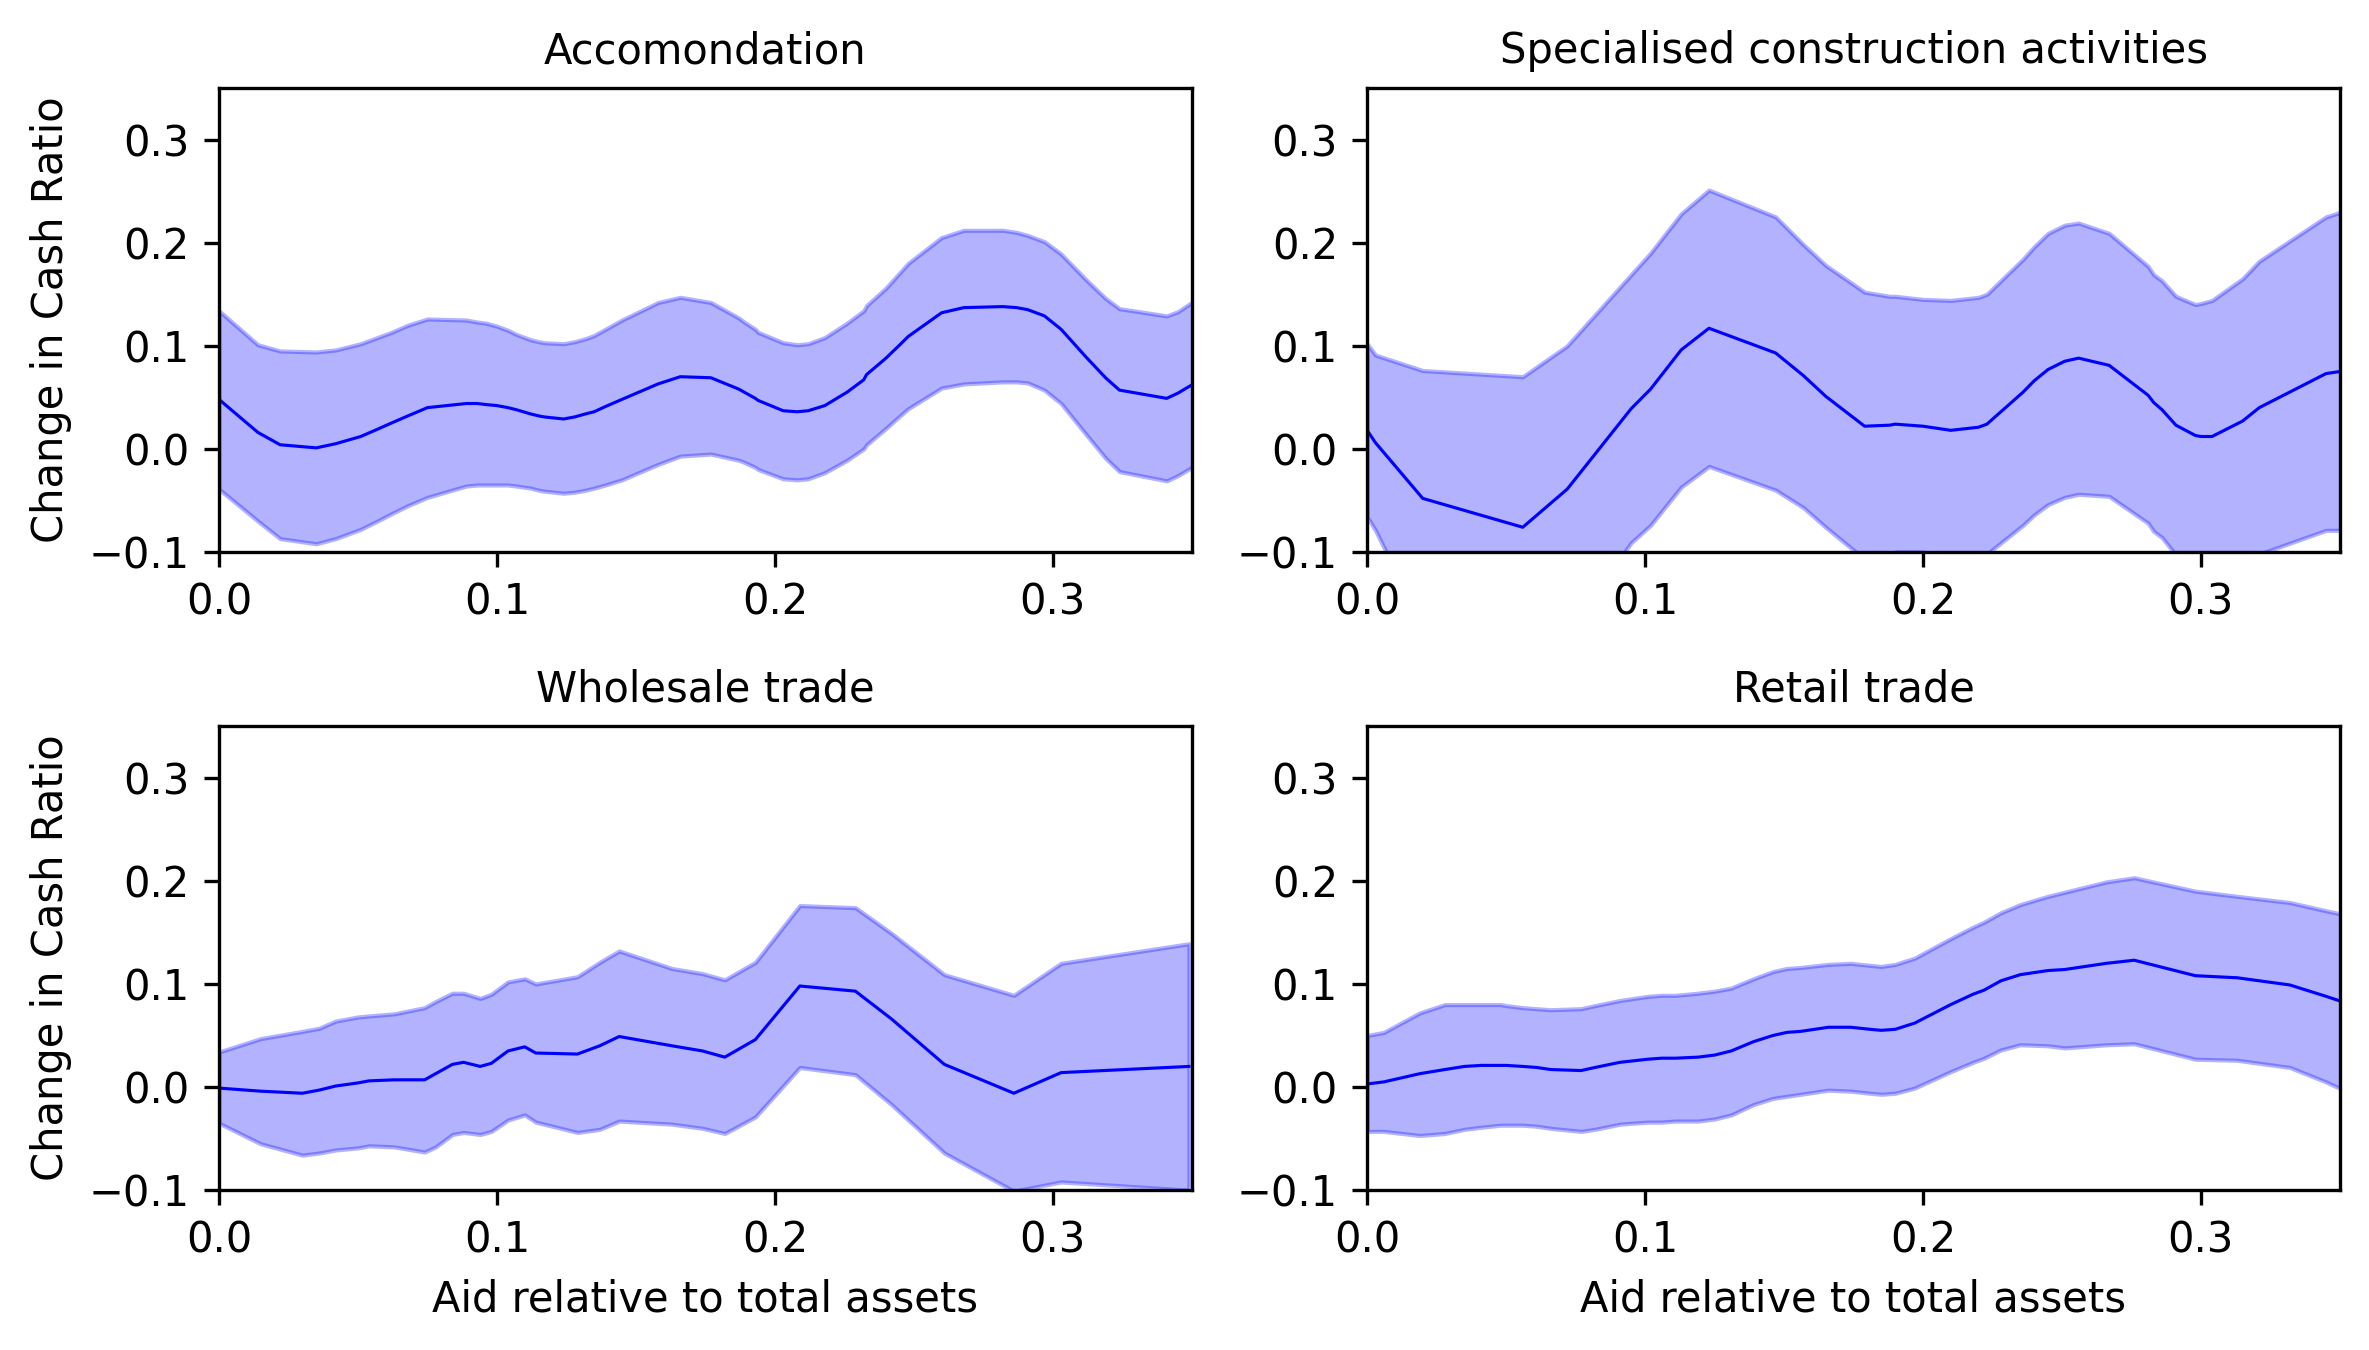
\includegraphics[width=1\columnwidth]{Figures/causal_curves_industries2.png}}
    
    \decoRule
    \caption[Response curves for liquidity through aid - by sectors 2]{Estimated Dose Response Functions, for the cash ratio from grants 2021 in selected industries in relative terms with 95\% Confidence Bands}
    \label{fig:Curve5}
\end{figure}

\begin{figure}
    \centering
    \makebox[\textwidth][c]{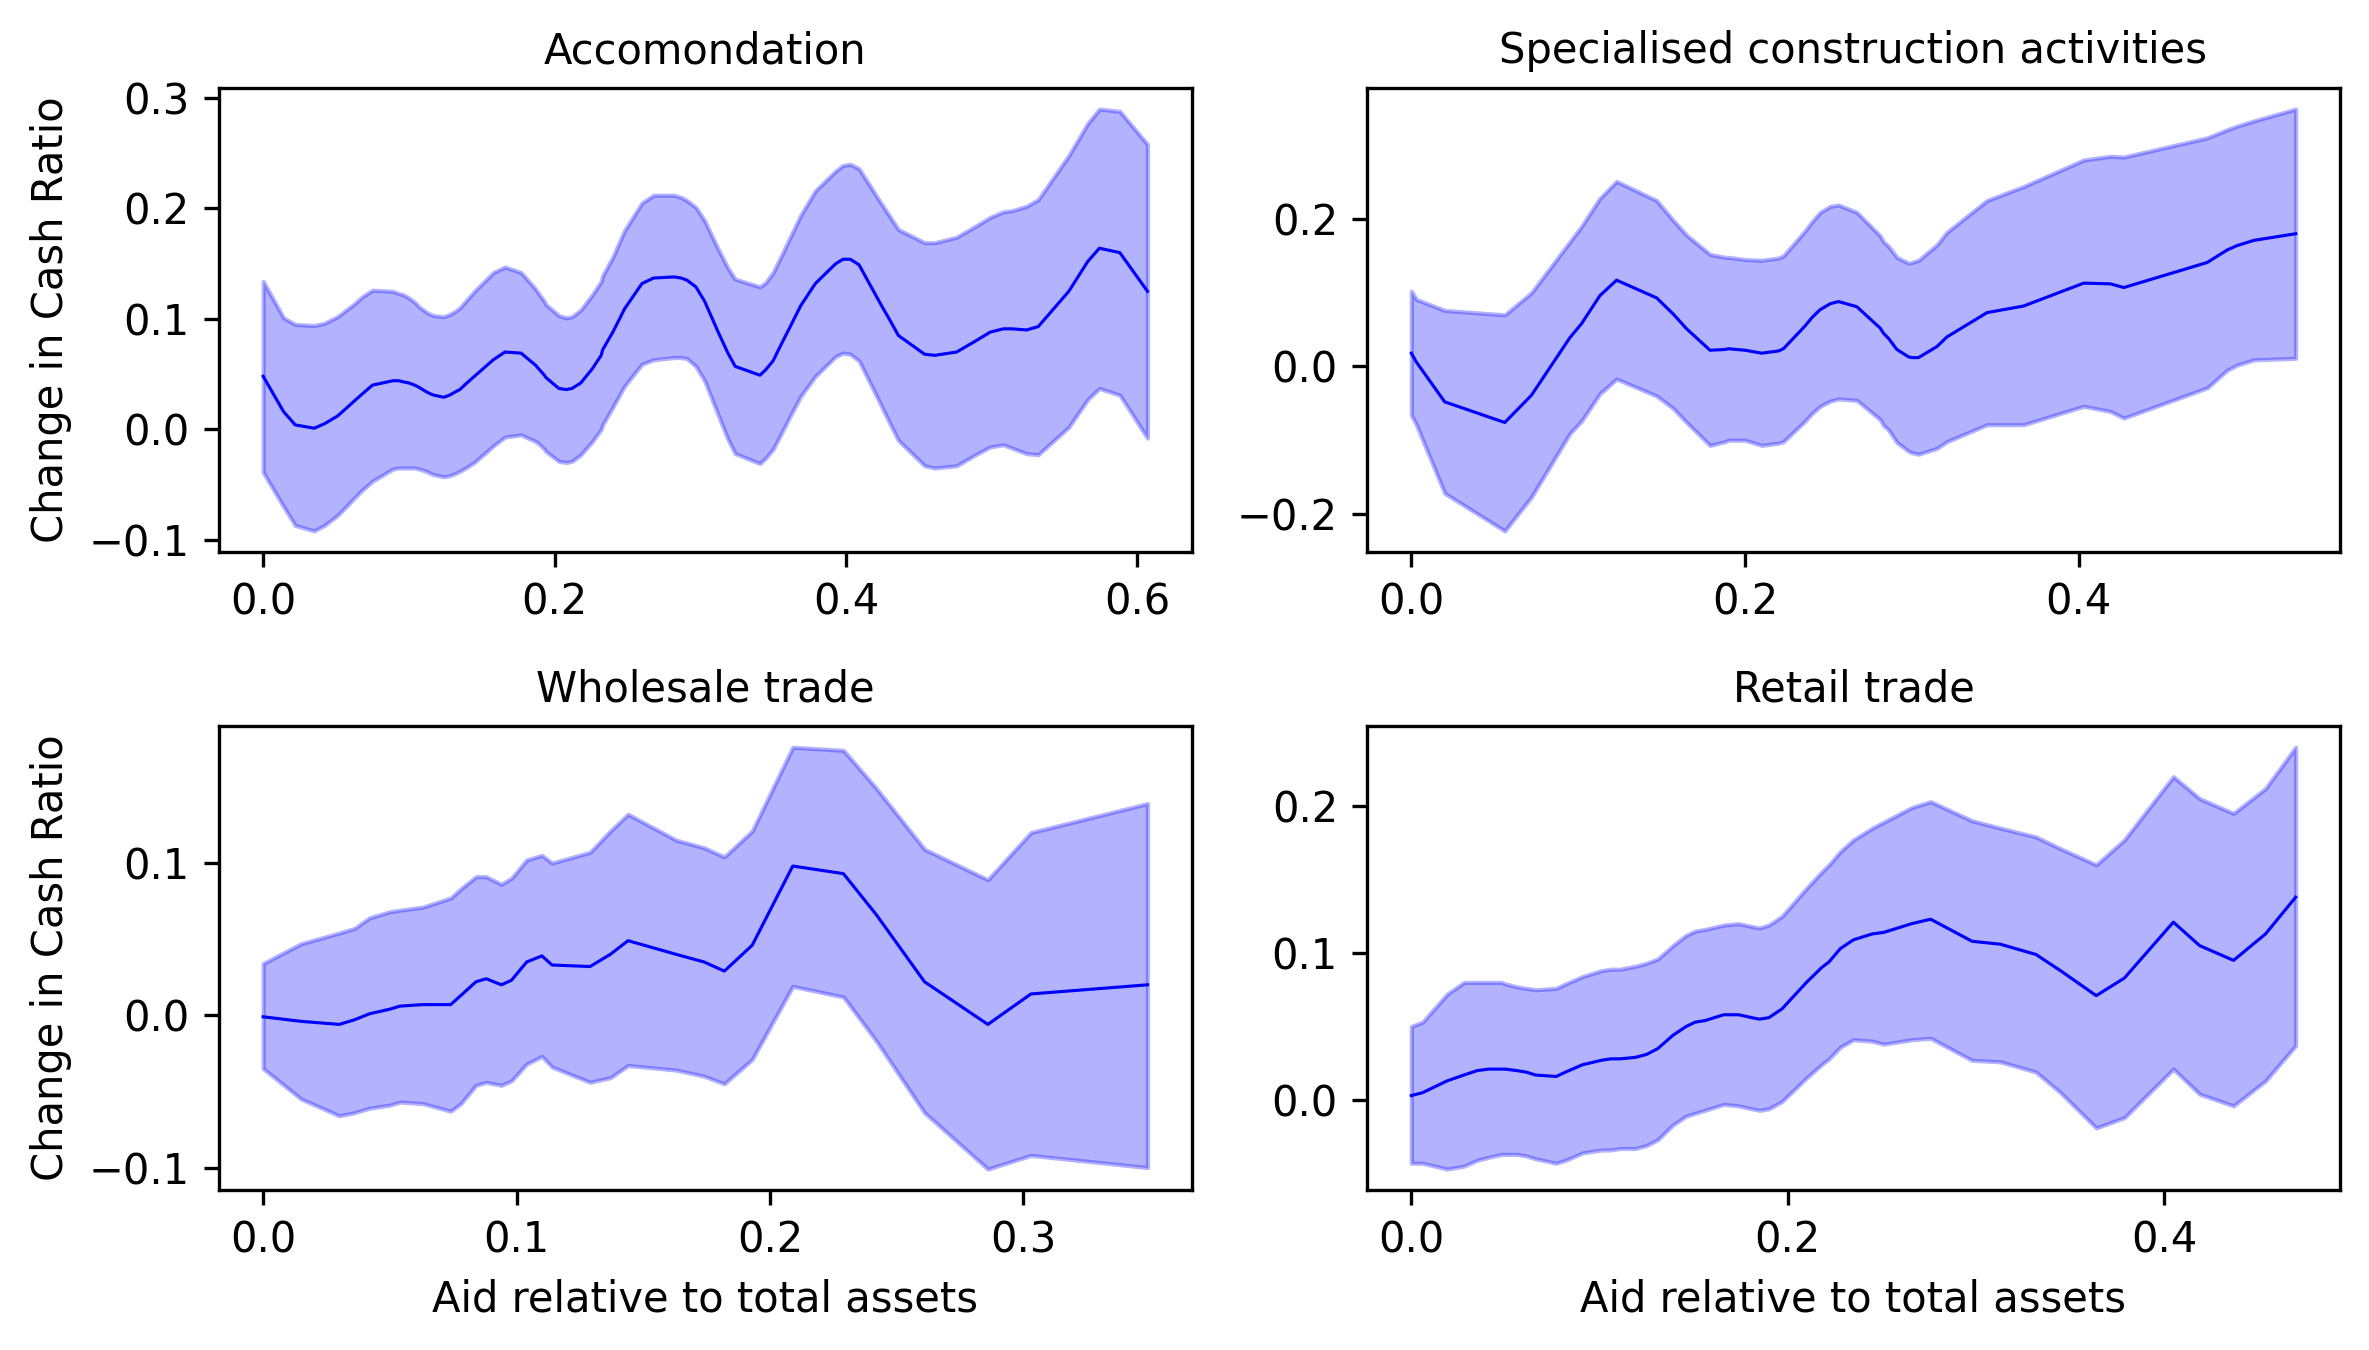
\includegraphics[width=1\columnwidth]{Figures/causal_curves_industries2_raw.png}}
    
    \decoRule
    \caption[Response curves for liquidity through aid - by sectors 2 uncut]{Estimated Dose Response Functions, for the cash ratio from grants 2021 in selected industries in relative terms with 95\% Confidence Bands}
    \label{fig:Curve5raw}
\end{figure}